

\tikzset{every picture/.style={line width=0.75pt}} %set default line width to 0.75pt        

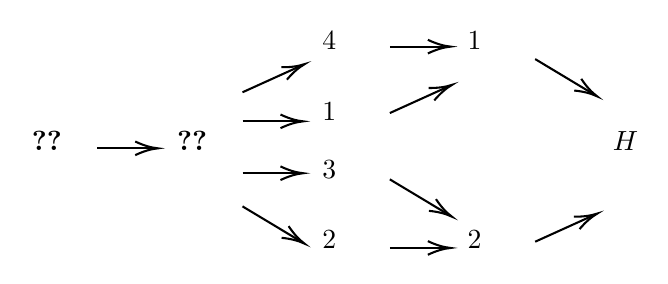
\begin{tikzpicture}[x=0.75pt,y=0.75pt,yscale=-1,xscale=1]
%uncomment if require: \path (0,260); %set diagram left start at 0, and has height of 260

%Straight Lines [id:da46892118468953903] 
\draw    (218.01,129) -- (245.25,129) ;
\draw [shift={(247.25,129)}, rotate = 180] [color={rgb, 255:red, 0; green, 0; blue, 0 }  ][line width=0.75]    (10.93,-3.29) .. controls (6.95,-1.4) and (3.31,-0.3) .. (0,0) .. controls (3.31,0.3) and (6.95,1.4) .. (10.93,3.29)   ;
%Straight Lines [id:da7558508357356156] 
\draw    (288.01,116) -- (315.25,116) ;
\draw [shift={(317.25,116)}, rotate = 180] [color={rgb, 255:red, 0; green, 0; blue, 0 }  ][line width=0.75]    (10.93,-3.29) .. controls (6.95,-1.4) and (3.31,-0.3) .. (0,0) .. controls (3.31,0.3) and (6.95,1.4) .. (10.93,3.29)   ;
%Straight Lines [id:da29220369712102556] 
\draw    (288.01,141) -- (315.25,141) ;
\draw [shift={(317.25,141)}, rotate = 180] [color={rgb, 255:red, 0; green, 0; blue, 0 }  ][line width=0.75]    (10.93,-3.29) .. controls (6.95,-1.4) and (3.31,-0.3) .. (0,0) .. controls (3.31,0.3) and (6.95,1.4) .. (10.93,3.29)   ;
%Straight Lines [id:da187430813346537] 
\draw    (288.01,102) -- (316.19,89.23) ;
\draw [shift={(318.01,88.4)}, rotate = 155.61] [color={rgb, 255:red, 0; green, 0; blue, 0 }  ][line width=0.75]    (10.93,-3.29) .. controls (6.95,-1.4) and (3.31,-0.3) .. (0,0) .. controls (3.31,0.3) and (6.95,1.4) .. (10.93,3.29)   ;
%Straight Lines [id:da021114195599838403] 
\draw    (288.01,156.96) -- (316.19,173.89) ;
\draw [shift={(317.9,174.93)}, rotate = 211.01] [color={rgb, 255:red, 0; green, 0; blue, 0 }  ][line width=0.75]    (10.93,-3.29) .. controls (6.95,-1.4) and (3.31,-0.3) .. (0,0) .. controls (3.31,0.3) and (6.95,1.4) .. (10.93,3.29)   ;
%Straight Lines [id:da21948815210536177] 
\draw    (359.01,177) -- (386.25,177) ;
\draw [shift={(388.25,177)}, rotate = 180] [color={rgb, 255:red, 0; green, 0; blue, 0 }  ][line width=0.75]    (10.93,-3.29) .. controls (6.95,-1.4) and (3.31,-0.3) .. (0,0) .. controls (3.31,0.3) and (6.95,1.4) .. (10.93,3.29)   ;
%Straight Lines [id:da339835070128927] 
\draw    (359.01,80) -- (386.25,80) ;
\draw [shift={(388.25,80)}, rotate = 180] [color={rgb, 255:red, 0; green, 0; blue, 0 }  ][line width=0.75]    (10.93,-3.29) .. controls (6.95,-1.4) and (3.31,-0.3) .. (0,0) .. controls (3.31,0.3) and (6.95,1.4) .. (10.93,3.29)   ;
%Straight Lines [id:da572960663012647] 
\draw    (359.01,112) -- (387.19,99.23) ;
\draw [shift={(389.01,98.4)}, rotate = 155.61] [color={rgb, 255:red, 0; green, 0; blue, 0 }  ][line width=0.75]    (10.93,-3.29) .. controls (6.95,-1.4) and (3.31,-0.3) .. (0,0) .. controls (3.31,0.3) and (6.95,1.4) .. (10.93,3.29)   ;
%Straight Lines [id:da5835932683194811] 
\draw    (359.01,143.96) -- (387.19,160.89) ;
\draw [shift={(388.9,161.93)}, rotate = 211.01] [color={rgb, 255:red, 0; green, 0; blue, 0 }  ][line width=0.75]    (10.93,-3.29) .. controls (6.95,-1.4) and (3.31,-0.3) .. (0,0) .. controls (3.31,0.3) and (6.95,1.4) .. (10.93,3.29)   ;
%Straight Lines [id:da42931684691427685] 
\draw    (429.01,86) -- (457.19,102.93) ;
\draw [shift={(458.9,103.97)}, rotate = 211.01] [color={rgb, 255:red, 0; green, 0; blue, 0 }  ][line width=0.75]    (10.93,-3.29) .. controls (6.95,-1.4) and (3.31,-0.3) .. (0,0) .. controls (3.31,0.3) and (6.95,1.4) .. (10.93,3.29)   ;
%Straight Lines [id:da6906806415816943] 
\draw    (429.01,174) -- (457.19,161.23) ;
\draw [shift={(459.01,160.4)}, rotate = 155.61] [color={rgb, 255:red, 0; green, 0; blue, 0 }  ][line width=0.75]    (10.93,-3.29) .. controls (6.95,-1.4) and (3.31,-0.3) .. (0,0) .. controls (3.31,0.3) and (6.95,1.4) .. (10.93,3.29)   ;


% Text Node
\draw (325.01,71.37) node [anchor=north west][inner sep=0.75pt]    {$\PPIVn{4}$};
% Text Node
\draw (325.01,105.4) node [anchor=north west][inner sep=0.75pt]    {$\PPIIIprn{1}$};
% Text Node
\draw (325.01,133.4) node [anchor=north west][inner sep=0.75pt]    {$\PPIVn{3}$};
% Text Node
\draw (325.01,167.4) node [anchor=north west][inner sep=0.75pt]    {$\PPIIIprn{2}$};
% Text Node
\draw (255.01,119.4) node [anchor=north west][inner sep=0.75pt]    {\ref{eq:P5_1}};
% Text Node
\draw (185.01,119.4) node [anchor=north west][inner sep=0.75pt]    {\ref{eq:P6_1}};
% Text Node
\draw (395.01,71.39) node [anchor=north west][inner sep=0.75pt]    {$\PPIIn{1}$};
% Text Node
\draw (395.01,167.4) node [anchor=north west][inner sep=0.75pt]    {$\PPIIn{2}$};
% Text Node
\draw (465.01,119.4) node [anchor=north west][inner sep=0.75pt]    {$\PIn{H}$};


\end{tikzpicture}